\section{Results}
    \subsection{Classification}

		The accurary score, F1-score, AUC-score and the gains-ratio of the classification neural network after studing the credit card data can be seen in figure \ref{fig:cc_acc}, \ref{fig:cc_F1}, \ref{fig:cc_auc} and \ref{fig:cc_gr} respectively.

		\begin{figure}[H]
			\centering
			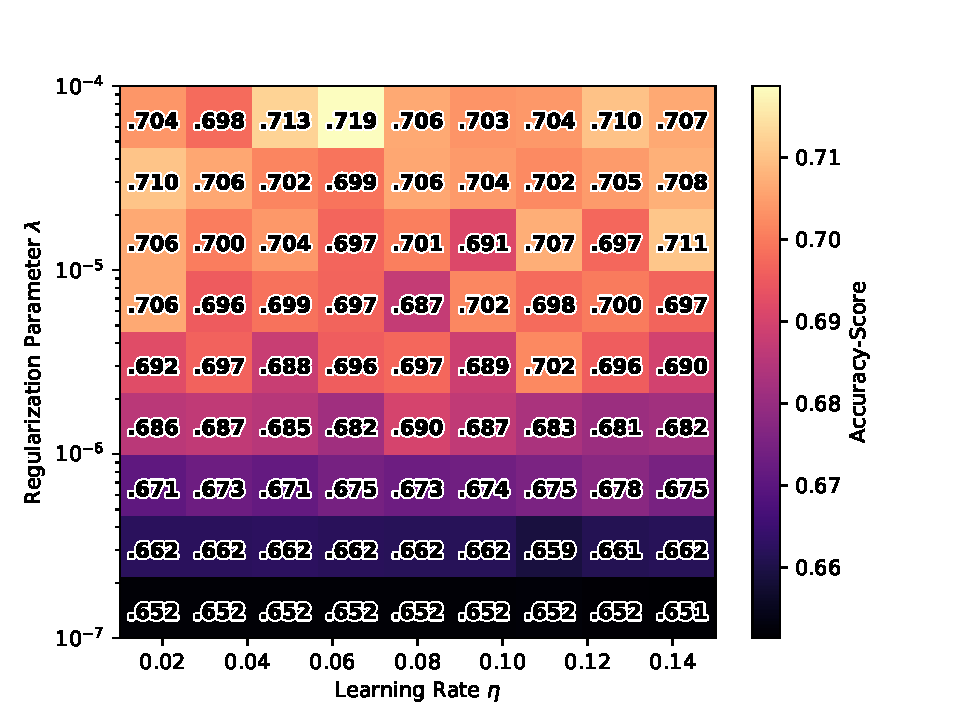
\includegraphics[width=0.5\textwidth]{figures/cc_res_0.pdf}
			\caption{The accurary score of the classification neural network for different $\eta$ and $\lambda$-values after studing the credit card data.}
			\label{fig:cc_acc}
		\end{figure}
		\begin{figure}[H]
			\centering
			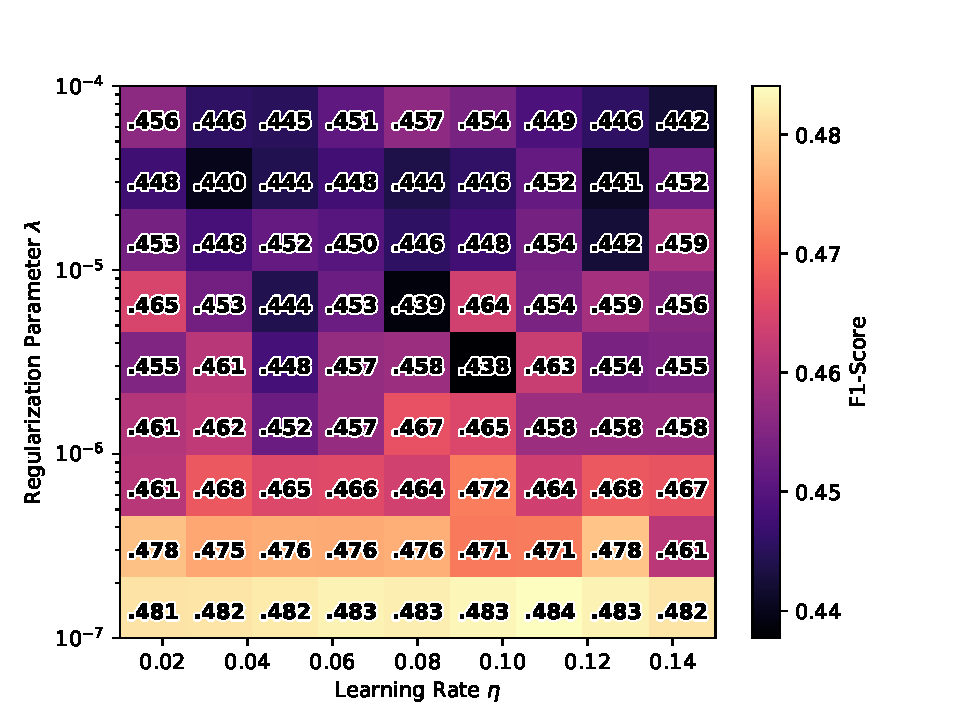
\includegraphics[width=0.5\textwidth]{figures/cc_res_1.pdf}
			\caption{The F1-score of the classification neural network for different $\eta$ and $\lambda$-values after studing the credit card data.}
			\label{fig:cc_F1}
		\end{figure}
		\begin{figure}[H]
			\centering
			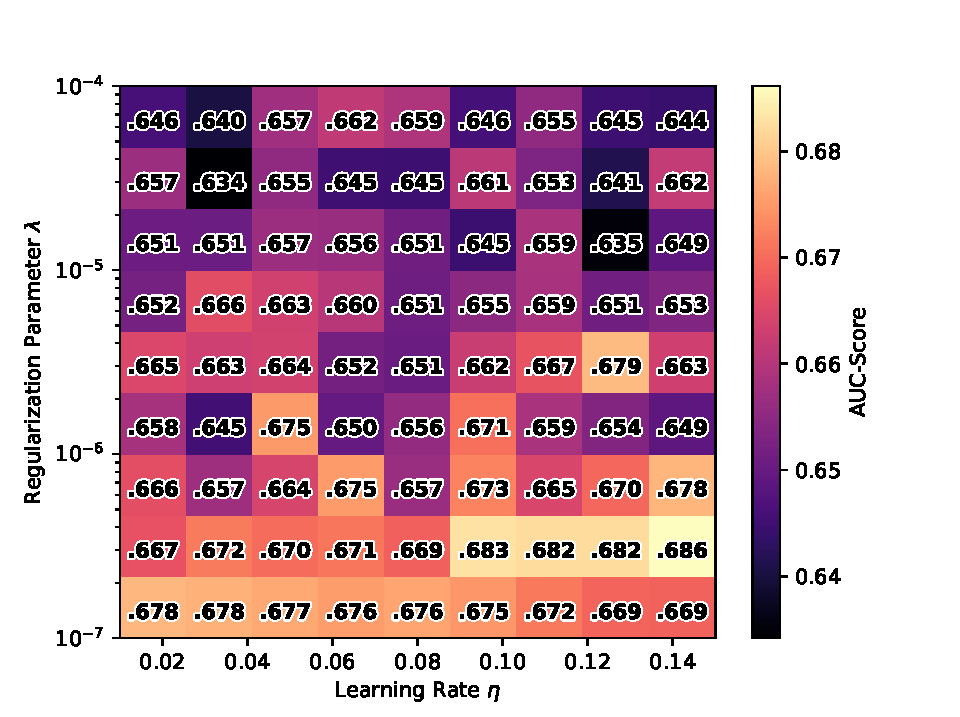
\includegraphics[width=0.5\textwidth]{figures/cc_res_2.pdf}
			\caption{The AUC-score of the classification neural network for different $\eta$ and $\lambda$-values after studing the credit card data.}
			\label{fig:cc_auc}
		\end{figure}
		\begin{figure}[H]
			\centering
			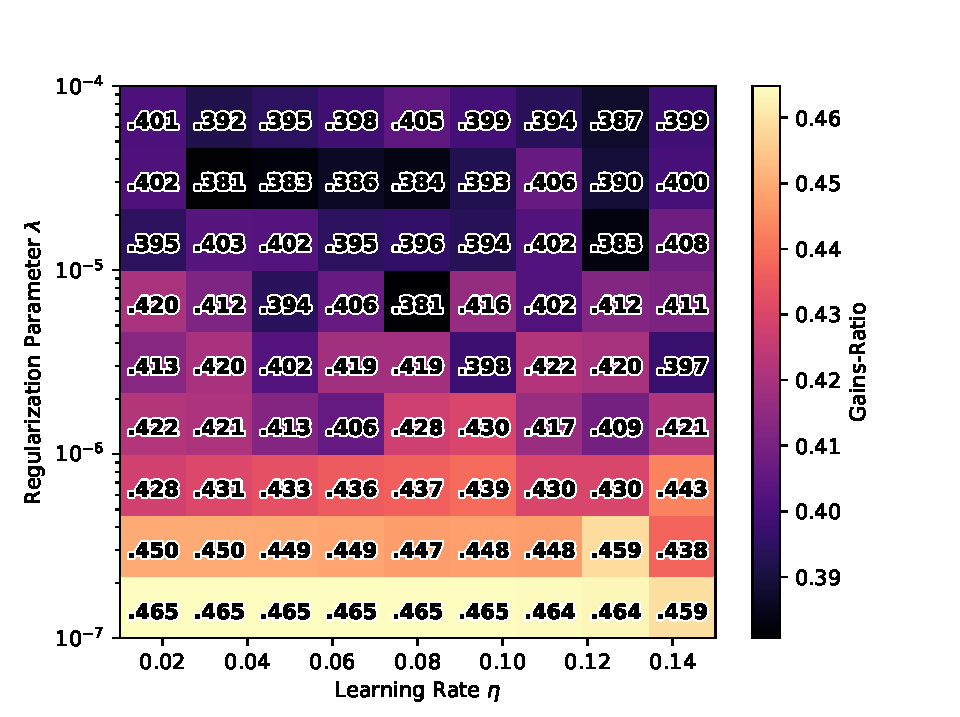
\includegraphics[width=0.5\textwidth]{figures/cc_res_3.pdf}
			\caption{The Gains-Ratio of the classification neural network for different $\eta$ and $\lambda$-values after studing the credit card data.}
			\label{fig:cc_gr}
		\end{figure}
	
        
        
    \subsection{Regression}
    
    	The mean squared error and the $R^2$-score of the regression neural network for different $\eta$ and $\lambda$-values after studing Franke's function can be seen in figure \ref{fig:ff_mse} and \ref{fig:ff_r2} respectively.
    
    	\begin{figure}[H]
    		\centering
    		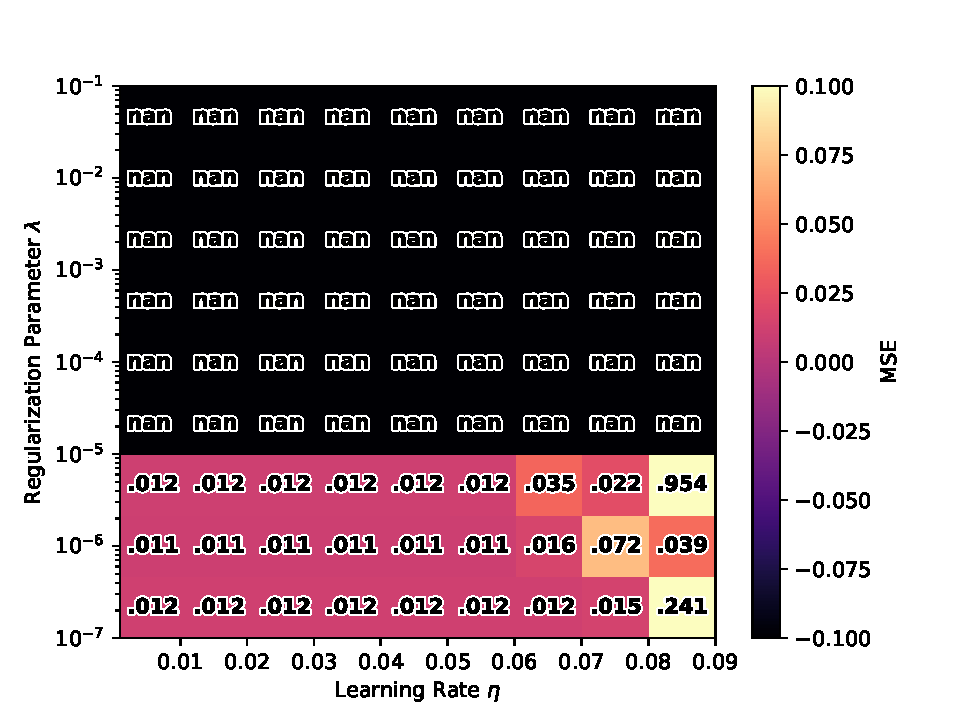
\includegraphics[width=0.5\textwidth]{figures/ff_res_0.pdf}
    		\caption{The mean squared error of the regression neural network for different $\eta$ and $\lambda$-values after studing Franke's function.}
    		\label{fig:ff_mse}
    	\end{figure}
    	\begin{figure}[H]
    		\centering
    		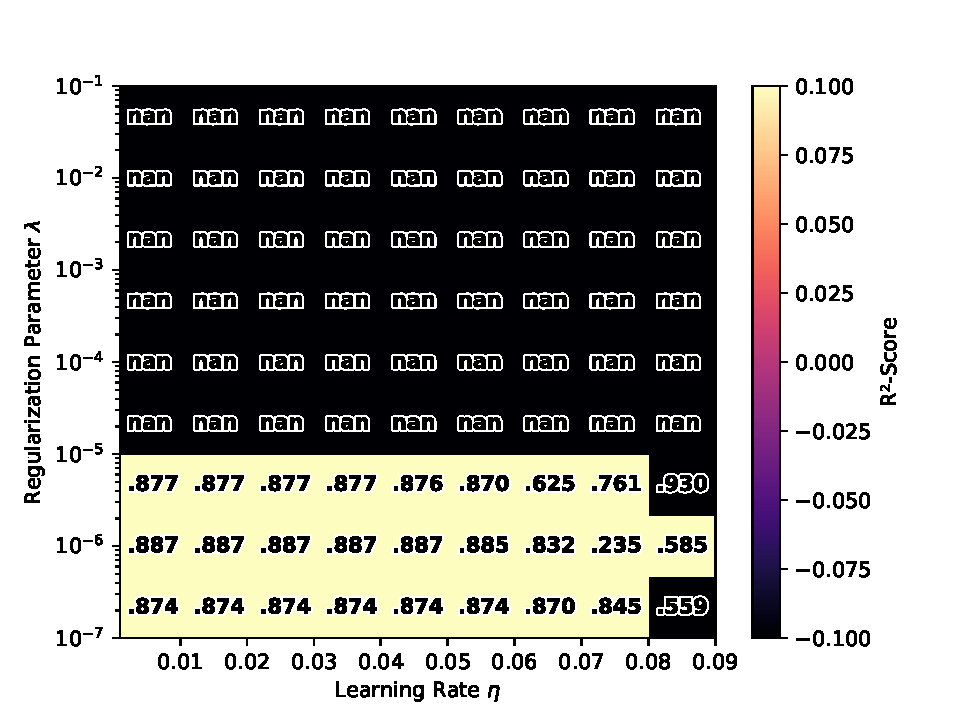
\includegraphics[width=0.5\textwidth]{figures/ff_res_1.pdf}
    		\caption{The $R^2$-score of the regression neural network after studing Franke's function.}
    		\label{fig:ff_r2}
    	\end{figure}
    
    
